\documentstyle[11pt,epsfig,fancybox,semcolor,semlayer,doublespace,portrait,rotate]
{seminar}
\input clp_utils

\def\ys{$\Upsilon(1S)$}
\def\yss{$\Upsilon(2S)$}
\def\ysss{$\Upsilon(3S)$}
\def\gamee{$\Gamma_{ee}$}
\def\hpqcd{{\sc Hpqcd}}
\def\argus{{\sc Argus}}
\def\cesr{{\sc Cesr}}
\def\cleo{{\sc Cleo}}
\def\cleoi{{\sc Cleo I}}
\def\cleoii{{\sc Cleo II}}
\def\cleoiii{{\sc Cleo III}}

% The following strings are needed by the title page and 
% page style definitions in map_utils.tex
\newcommand{\talktitle}[0]{\gamee\ of \ys, \yss\ and \ysss}
\newcommand{\fmttitle}[0]{}
\newcommand{\conftitle}[0]{Cargese School of Particle Physics and Cosmology}
\newcommand{\myname}[0]{Jim Pivarski}
\newcommand{\affila}[0]{Cornell University, \cleo\ Collaboration}
\newcommand{\talkdate}[0]{August 15, 2003}

\pagestyle{conference}   % From clp_utils.tex

% slide magnification
\slidesmag 1

%%%%%%%%%%%%%%%%%%%%%%%%%%%%%%%%%%%%%%%%%%%%%%%%%%%%%%%%%%%%%%%%%%%%%%%%%%%
% Start document
\begin{document}

% Set page size
\slideheight 7.0in
\slidewidth 8.8in 

% Set array stretch
\renewcommand{\arraystretch}{0.3}
\renewcommand{\slidetopmargin}{0.4in}
\renewcommand{\slidebottommargin}{0.9in}


%%%%%%%%%%%%%%%%%%%%%%%%%%%%%%%%%%%%%%%%%%%%%%%%%%%%%%%%%%%%%%%%%%%%%%%%%%%

\begin{slide*}

\slideframe{}
\slideframe*[\dkblue]{Oval}

\begin{center}
\vspace{4 cm}
{\Huge \gamee\ (Leptonic Decay Width) \\
\vspace{0.5 cm} of \ys, \yss\  and \ysss}  \\
\vspace{1 cm}
\begin{center}
  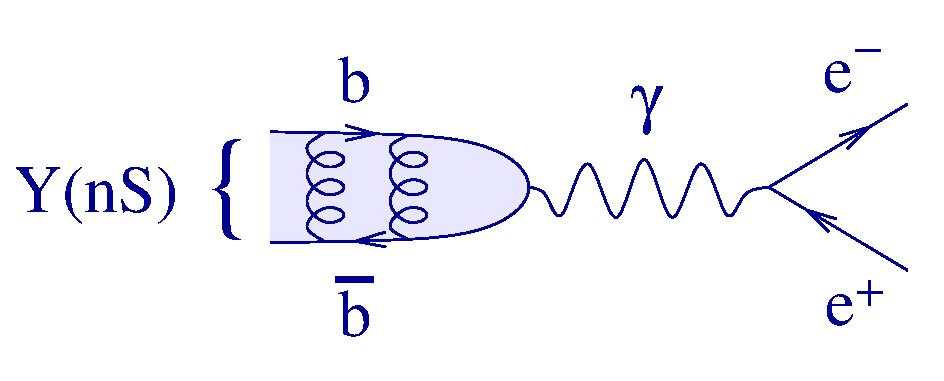
\epsfig{file=gamee_diagram.eps, width=0.8\linewidth}
\end{center}
\vspace{1 cm}
{\LARGE	Jim Pivarski } \\
% \vspace{0.25 cm}
% {\LARGE	Ritchie Patterson } \\
% \vspace{0.25 cm}
% {\LARGE	Karl Berkelman } \\
\vspace{0.25 cm}
{\LARGE	Cornell University } \\
\vspace{1 cm}
{\LARGE	\cleo\  Collaboration } \\
\vspace{2 cm}
\LARGE Cargese School of Particle Physics and Cosmology \\
{\LARGE \talkdate}

\end{center}

\end{slide*}

% %%%%%%%%%%%%%%%%%%%%%%%%%%%%%%%%%%%%%%%%%%%%%%%%%%%%%%%%%%%%%%%%%%%%%%%%%%%

\begin{slide*}
\slideframe{}
\slideframe*[\dkblue]{Oval}
\heading{\huge Motivation: from Lattice QCD}
\begin{minipage}[t]{\linewidth}

\vspace{0.3 cm}
\begin{center}
  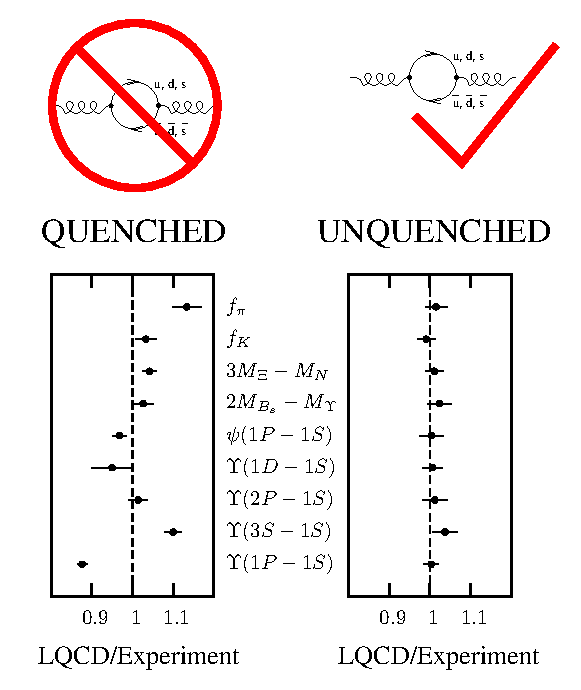
\epsfig{file=lqcd_success2.eps, width=0.9\linewidth}
\end{center}

\end{minipage}
\end{slide*}

%%%%%%%%%%%%%%%%%%%%%%%%%%%%%%%%%%%%%%%%%%%%%%%%%%%%%%%%%%%%%%%%%%%%%%%%%%%

\begin{slide*}
\slideframe{}
\slideframe*[\dkblue]{Oval}
\begin{minipage}[t]{\linewidth}
\LARGE \black

\begin{enumerate}

  \item Non-perturbative QCD can be subjected to precision tests

  \item LQCD calculations can be used to calculate semileptonic form
  factors (and extract CKM matrix elements)

  \item \ldots

\end{enumerate}

\vspace{0.5 cm}
\heading{\huge \gamee\ of \ys, \yss, \ysss}
\vspace{0.7 cm}

\begin{center}
  \begin{tabular}{p{0.28\linewidth} p{0.04\linewidth} p{0.52\linewidth}}
    \begin{minipage}{\linewidth}
      \begin{center}
        \huge $\Gamma(\Upsilon \to e^+e^-)$
      \end{center}
    \end{minipage} &
    \begin{minipage}{\linewidth}
      \begin{center}
        \huge $\sim$
      \end{center}
    \end{minipage} &
    \begin{minipage}{\linewidth}
      \begin{center}
        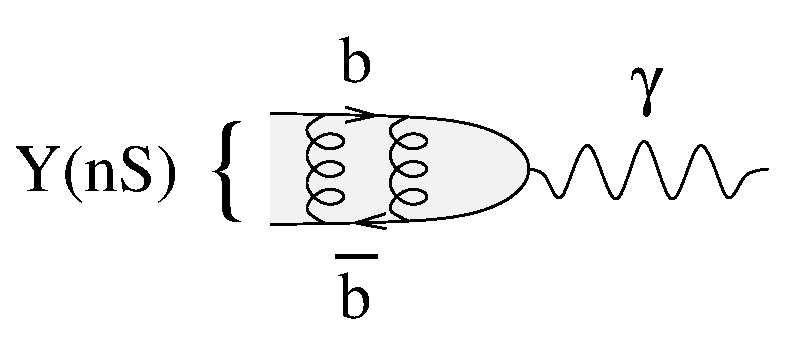
\epsfig{file=gamee_diagram3.eps, width=\linewidth}
      \end{center}
    \end{minipage}
  \end{tabular}
  \vspace{0.2 cm}
  \begin{tabular}{p{0.28\linewidth} p{0.04\linewidth} p{0.52\linewidth}}
    \begin{minipage}{\linewidth}
      \begin{center}
        \huge $f_B$
      \end{center}
    \end{minipage} &
    \begin{minipage}{\linewidth}
      \begin{center}
        \huge $\sim$
      \end{center}
    \end{minipage} &
    \begin{minipage}{\linewidth}
      \begin{center}
        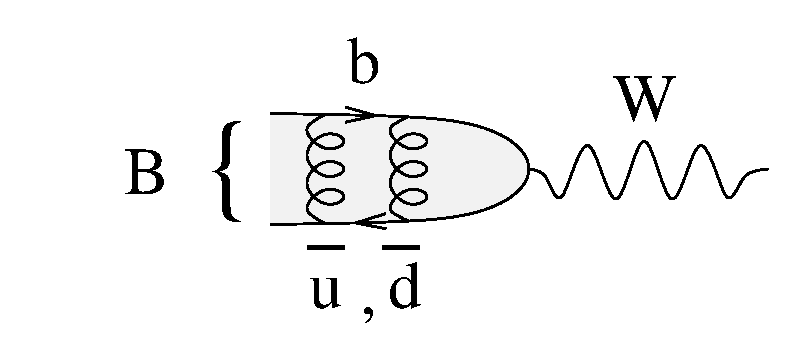
\epsfig{file=fb_diagram3.eps, width=\linewidth}
      \end{center}
    \end{minipage}
  \end{tabular}
\end{center}

\vspace{0.6 cm}
\fbox{\begin{minipage}{0.8\linewidth}
  \vspace{0.2 cm}
  \begin{center}
    \Huge \gamee\ calculation is underway, \\
    with a goal of 3\% $\delta(\Gamma_{ee})/\Gamma_{ee}$
  \end{center}
  \vspace{0.2 cm}
\end{minipage}}

%% \vspace{1.5 cm}
%% \begin{minipage}{\linewidth}
%%   \gamee\ calculation is underway, with a goal of 3\% $\sigma_{\Gamma_{ee}}/\Gamma_{ee}$:
%%   \vspace{0.5 cm}
%%   \begin{center}
%%     \fbox{\begin{minipage}{0.9\linewidth}
%% 	\begin{center}
%% 	  \Large
%% 	      {\bf The Upsilon spectrum from lattice QCD with 2+1 flavors of dynamical quarks} \\
%% 	      A.~Gray {\it et al.}  [HPQCD collaboration] \\
%% 	      \LARGE \tt arXiv:hep-lat/0209022
%% 	\end{center}
%%     \end{minipage}}
%%   \end{center}
%% \end{minipage}

\end{minipage}
\end{slide*}

%%%%%%%%%%%%%%%%%%%%%%%%%%%%%%%%%%%%%%%%%%%%%%%%%%%%%%%%%%%%%%%%%%%%%%%%

\begin{slide*}
\slideframe{}
\slideframe*[\dkblue]{Oval}
\rotate[r]{\mbox{
\begin{minipage}[t]{\textheight}
\vspace{-0.74\textheight}
\heading{\huge Experimental Status of \gamee}
\LARGE \black
\begin{tabular}{p{0.17\linewidth} p{0.23\linewidth} p{0.23\linewidth} p{0.23\linewidth}}
  &
  \begin{center} \LARGE $\Upsilon(1S)$ \end{center} &
  \begin{center} \LARGE $\Upsilon(2S)$ \end{center} &
  \begin{center} \LARGE $\Upsilon(3S)$ \end{center}
\end{tabular}
\vspace{-1 cm}
\begin{center}
  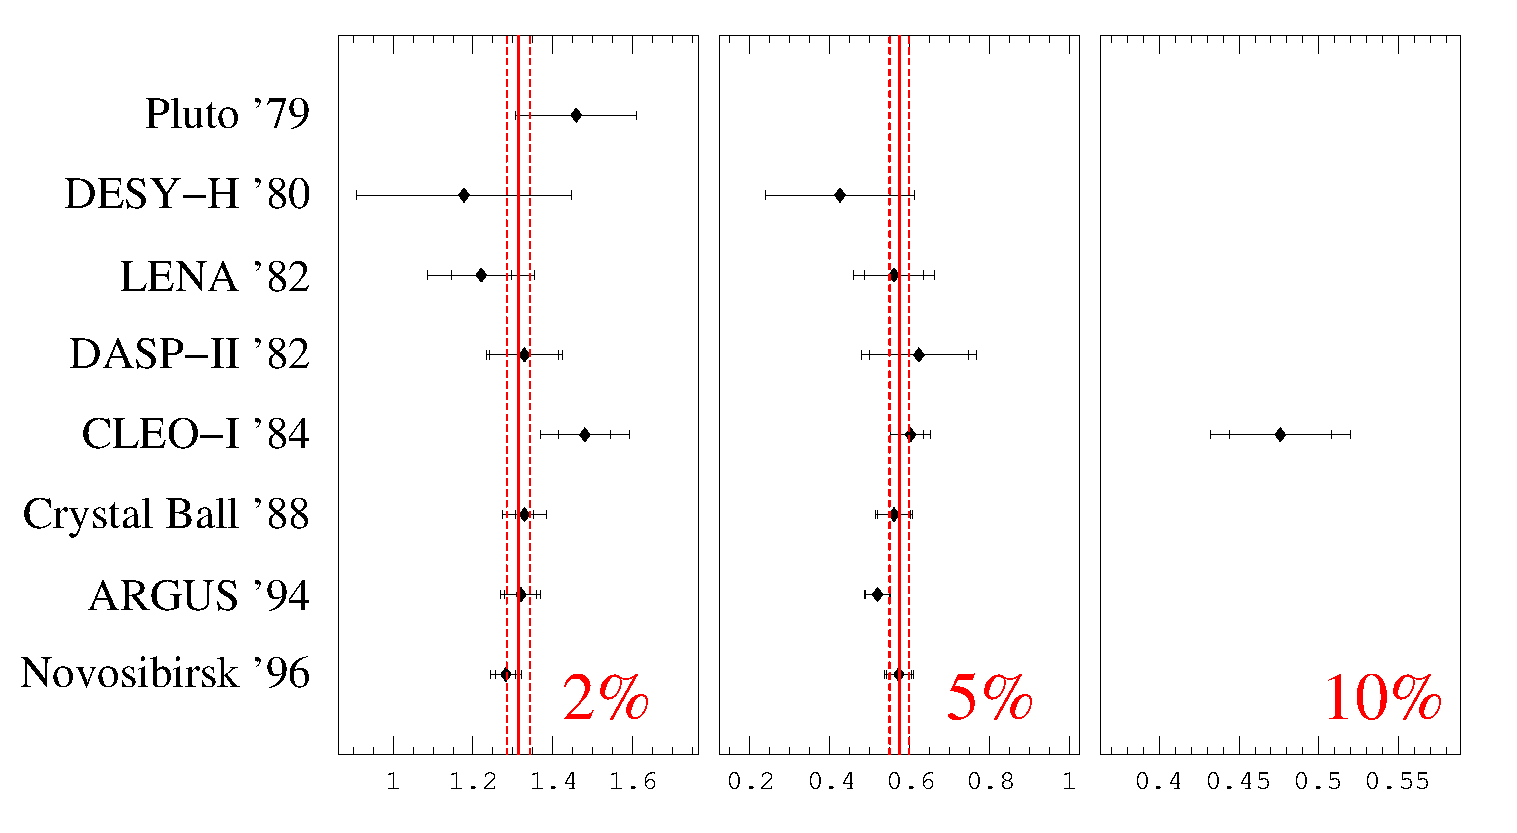
\epsfig{file=pdg_plots2.eps, width=\linewidth}
\end{center}
\vspace{-0.9 cm}
\begin{tabular}{p{0.17\linewidth} p{0.23\linewidth} p{0.23\linewidth} p{0.23\linewidth}}
  &
  \begin{center} \LARGE \gamee\ (keV) \end{center} &
  \begin{center} \LARGE \gamee\ (keV) \end{center} &
  \begin{center} \LARGE \gamee\ (keV) \end{center}
\end{tabular}
\end{minipage}}}
\end{slide*}

%%%%%%%%%%%%%%%%%%%%%%%%%%%%%%%%%%%%%%%%%%%%%%%%%%%%%%%%%%%%%%%%%%%%%%%%

\begin{slide*}
\slideframe{}
\slideframe*[\dkblue]{Oval}
\heading{\huge \cesr/\cleo\ Program to Measure \gamee}
\begin{minipage}[t]{\linewidth}
\LARGE \black

\vspace{0.5 cm}
\begin{itemize}

  \item Goal of 1--2\% uncertainty for all three resonances

  \vspace{0.5 cm}
  \item Measure {\red $\Gamma(\Upsilon \to e^+e^-)$}
        using {\blue $\sigma(e^+e^- \to \Upsilon)$:}

\begin{center}
  \[ {\red \Gamma(\Upsilon \to e^+ e^-)} = \frac{\mbox{$M_\Upsilon$}^2}{6 \pi^2} \mbox{ }
     \frac{\Gamma_{\mbox{\normalsize tot}}}{\Gamma_{\mbox{\normalsize had}}} \mbox{ }
     {\blue \int dE\, \sigma(e^+ e^- \to \Upsilon \to \mbox{hadrons})}
  \]
\end{center}

  \vspace{0.5 cm}
  \item Scan beam energy across resonance and plot hadronic cross-section

\vspace{0.5 cm}
\begin{center}
  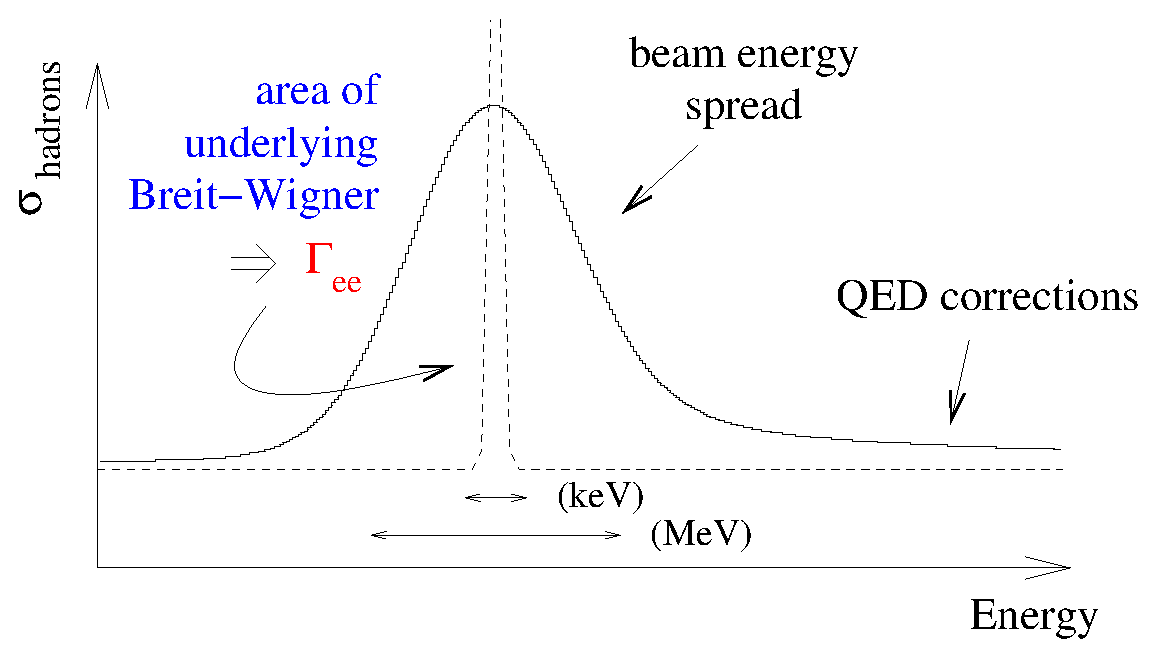
\epsfig{file=cartoon.eps, width=\linewidth}
\end{center}

\end{itemize}

\gray
\vspace{-1 cm}

%% \begin{tabular}{p{\linewidth}}
%%   \mbox{\hspace{\linewidth}} \\\hline
%% \end{tabular}

%% \vspace{0.1 cm}
%% \begin{center}
%% \begin{minipage}{0.9\linewidth}
%%     Why {\it hadronic} cross-section?
%%     \begin{itemize}
  
%%       \item ${\mathcal B}_{\mbox{\normalsize hadrons}}$ is large and known:
%% 	${\mathcal B}_{\mbox{\normalsize hadrons}} = 1 - 3 {\mathcal B}_{\ell\ell} \approx$ 94\%

%%       \item $e^+e^- \to \Upsilon \to \ell^+\ell^-$ interferes with $e^+e^- \to q\bar{q} \to \ell^+\ell^-$

%%       \item A measurement of ${\mathcal B}_{\ell\ell}$ will be made with the same data

%%     \end{itemize}
%%   \end{minipage}
%% \end{center}

\end{minipage}
\end{slide*}

%%%%%%%%%%%%%%%%%%%%%%%%%%%%%%%%%%%%%%%%%%%%%%%%%%%%%%%%%%%%%%%%%%%%%%%%

\begin{slide*}
\slideframe{}
\slideframe*[\dkblue]{Oval}
\heading{\huge \cleoiii\ Data}
\begin{minipage}[t]{\linewidth}
\LARGE \black

\begin{center}
  \begin{tabular}{p{0.02\linewidth} p{0.9\linewidth}}
    \begin{minipage}{\linewidth}
      \rotate[l]{\mbox{$\sigma(e^+e^- \to \mbox{hadrons})$ (nb)}}
    \end{minipage} &
    \begin{minipage}{\linewidth}
      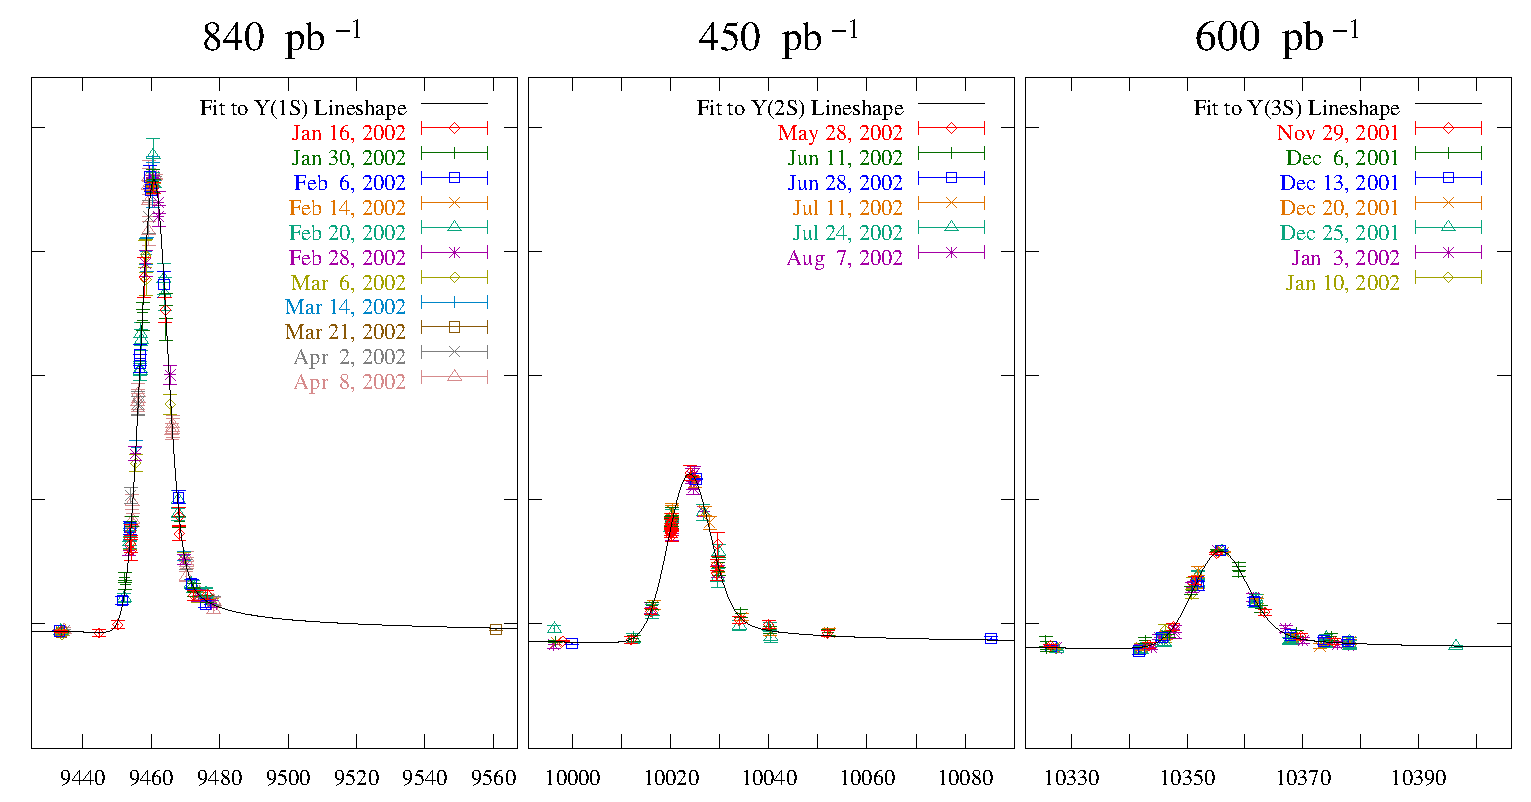
\epsfig{file=data.eps, width=\linewidth}
    \end{minipage} \\
    & \centering Energy (MeV)
  \end{tabular}
  \begin{minipage}{\linewidth}
    \vspace{-4 cm}
    \begin{tabular}{p{0.3\linewidth} p{0.3\linewidth} p{0.3\linewidth}}
      \centering \large \ys & \centering \large \yss & \centering \large \ysss
    \end{tabular}
  \end{minipage}
\end{center}

\vspace{1 cm}

\end{minipage}
\heading{\huge Best Before \cleoiii}
\begin{minipage}[t]{\linewidth}
\Large \black

\begin{center}
  \begin{tabular}{p{0.3\linewidth} p{0.3\linewidth} p{0.3\linewidth}}
    \begin{minipage}{\linewidth}
      \begin{center}
	Novosibirsk '96
      \end{center}
    \end{minipage} &
    \begin{minipage}{\linewidth}
      \begin{center}
	\argus\ '94
      \end{center}
    \end{minipage} &
    \begin{minipage}{\linewidth}
      \begin{center}
	\cleoi\ '84
      \end{center}
    \end{minipage}
  \end{tabular}
  \begin{tabular}{p{0.3\linewidth} p{0.3\linewidth} p{0.3\linewidth}}
    \begin{minipage}{\linewidth}
      \begin{center}
	\epsfig{file=novo_y1s.eps, width=\linewidth, height=\linewidth}
      \end{center}
    \end{minipage} &
    \begin{minipage}{\linewidth}
      \begin{center}
	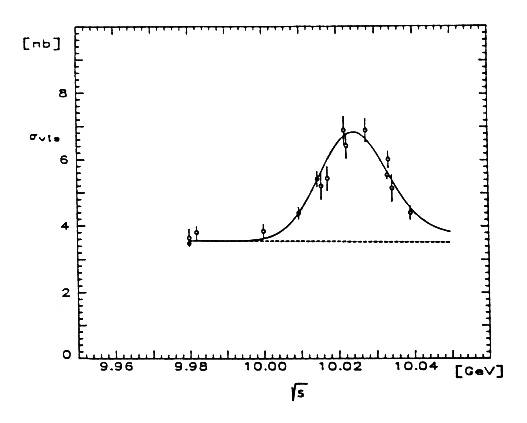
\epsfig{file=argus_y2s.eps, width=\linewidth, height=\linewidth}
      \end{center}
    \end{minipage} &
    \begin{minipage}{\linewidth}
      \begin{center}
	\epsfig{file=cleo1_y3s.eps, width=\linewidth, height=\linewidth}
      \end{center}
    \end{minipage}
  \end{tabular}
  \begin{minipage}{\linewidth}
    \vspace{-7 cm}
    \begin{tabular}{p{0.3\linewidth} p{0.3\linewidth} p{0.3\linewidth}}
      \centering \large \ys \hspace{1 cm} & \centering \large \yss & 
    \end{tabular}
  \end{minipage}
\end{center}

\vspace{0.5 cm}

\end{minipage}
\end{slide*}

%%%%%%%%%%%%%%%%%%%%%%%%%%%%%%%%%%%%%%%%%%%%%%%%%%%%%%%%%%%%%%%%%%%%%%%%%%

\begin{slide*}
\slideframe{}
\slideframe*[\dkblue]{Oval}
\heading{\huge Sources of Error}
\begin{minipage}[t]{\linewidth}
\Large \black

\begin{flushright}
  \begin{minipage}{5 cm}
    \begin{center}
      \begin{tabular}{c}
        \ys, \yss, \ysss \\\hline
      \end{tabular}
    \end{center}
  \end{minipage}
\end{flushright}

\vspace{0.5 cm}
$\surd$ Statistics
\vspace{-0.9 cm}
\begin{flushright}
  \begin{minipage}{4 cm}
    \begin{center}
	% currently 0.4\%, 0.5\%, 1.1\% \\
	0.1\%, 0.2\%, 0.4\%
    \end{center}
  \end{minipage}
\end{flushright}

\vspace{0.9 cm}
$\surd$ Backgrounds
\vspace{-0.9 cm}
\begin{flushright}
  \begin{minipage}{4 cm}
    \begin{center}
      0.2\%, 0.2\%, 0.1\%
    \end{center}
  \end{minipage}
\end{flushright}

\vspace{0.2 cm} \hspace{0.6 cm} \begin{tabular}{c l}
  $\surd$ & Selection Criteria Chosen \\
  $\surd$ & Backgrounds Measured to be Small
\end{tabular}

\vspace{0.9 cm}
$\rightarrow$ Efficiency
\vspace{-1.3 cm}
\begin{flushright}
  currently 1.0\%, 1.5\%, 1.7\% \\
  best-case 0.4\%, 0.4\%, 0.5\%
\end{flushright}

\vspace{0.2 cm} \hspace{0.6 cm} \begin{tabular}{c l}
  $\surd$ & Estimated with Monte Carlo \\
  $\rightarrow$ & Reduce systematic errors
\end{tabular}

\vspace{0.9 cm}
$\rightarrow$ Luminosity
\vspace{-1.3 cm}
\begin{flushright}
  currently 2.5\% \\
  goal of 1.0\%
\end{flushright}

\vspace{0.2 cm} \hspace{0.6 cm} \begin{tabular}{c l}
  $\surd$ & Measured with $e^+e^- \to \gamma \gamma$ \\
  $\rightarrow$ & Measure with $\to e^+e^-$ and $\to \mu^+\mu^-$ also
\end{tabular}

\vspace{0.9 cm}
$\rightarrow$ Energy
\vspace{-0.9 cm}
\begin{flushright}
  currently 1.0\%
\end{flushright}

\vspace{0.2 cm} \hspace{0.6 cm} \begin{tabular}{c l}
  $\surd$ & Scanned each peak many times for cross-checks \\
  $\rightarrow$ & Reduce upper limit on calibration stability \\
\end{tabular}

\vspace{0.2 cm}

\end{minipage}
\end{slide*}

%%%%%%%%%%%%%%%%%%%%%%%%%%%%%%%%%%%%%%%%%%%%%%%%%%%%%%%%%%%%%%%%%%%%%%%

\begin{slide*}
\slideframe{}
\slideframe*[\dkblue]{Oval}
\begin{minipage}[t]{\linewidth}
\Large \black

{
  \dkblue
  \begin{tabular}{c c c c}
    \hspace{0.25 cm} \fbox{Backgrounds} \hspace{0.25 cm} &
    \hspace{0.25 cm} \mbox{Efficiency} \hspace{0.25 cm} &
    \hspace{0.25 cm} \mbox{Luminosity} \hspace{0.25 cm} &
    \hspace{0.25 cm} \mbox{Energy} \hspace{0.25 cm} \\
    $\Downarrow$ & & & \\
  \end{tabular}
}

\vspace{-0.2 cm}
\begin{tabular}{c l}
  $\surd$ & Selection Criteria Chosen \\
  $\surd$ & Backgrounds Measured to be Small
\end{tabular}

\LARGE

\vspace{0.5 cm}
\begin{tabular}{p{0.02\linewidth} p{0.9\linewidth}}
  \begin{minipage}{\linewidth}
    \rotate[l]{\mbox{$\sigma(e^+e^- \to \mbox{hadrons})$ (nb)}}
  \end{minipage} &
  \begin{minipage}{\linewidth}
    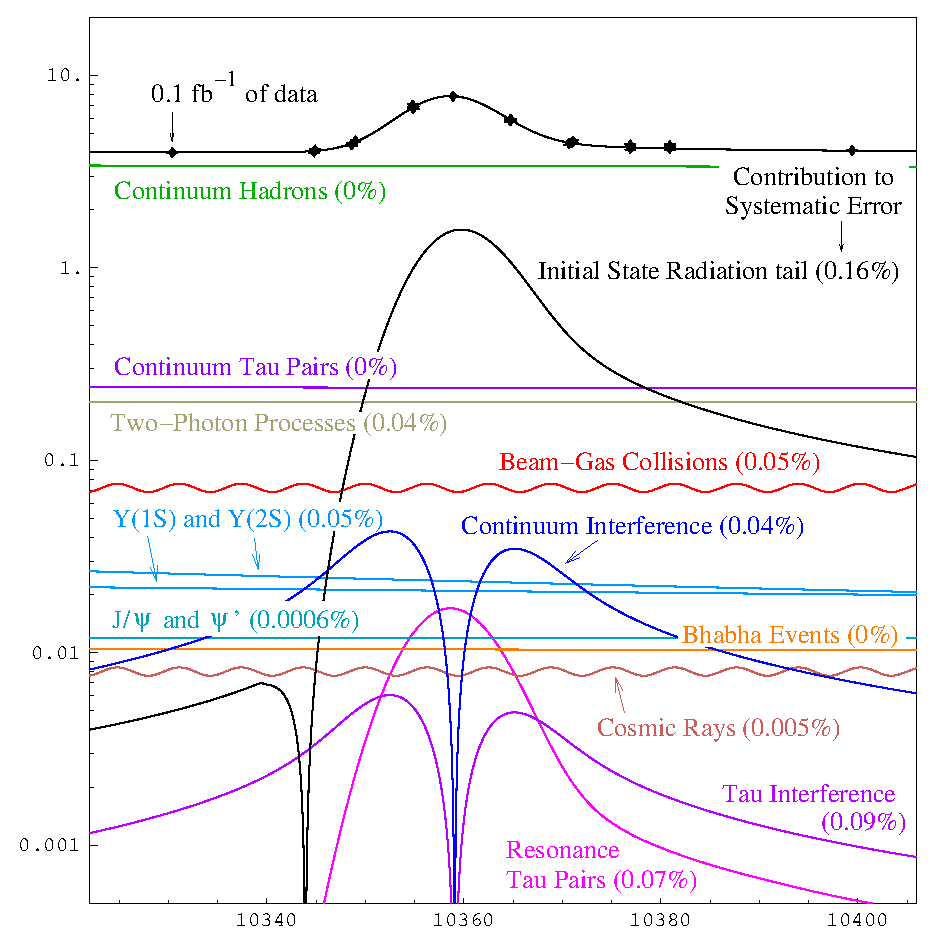
\epsfig{file=backgrounds_withISRtail_wtau.eps, width=\linewidth}
  \end{minipage} \\
  & \centering Energy (MeV)
\end{tabular}
\vspace{-0.5 cm}

%% \vspace{0.4 cm}
%% \begin{minipage}{\linewidth}
%%   \normalsize
%%   \begin{tabular}{p{6cm} c c c}
%%     Contribution to Fractional Error
%%     & \hspace{0.07 cm} $\Gamma_{ee}\left(\mbox{\ys}\right)$ \hspace{0.07 cm}
%%     & \hspace{0.07 cm} $\Gamma_{ee}\left(\mbox{\yss}\right)$ \hspace{0.07 cm}
%%     &  \hspace{0.07 cm} $\Gamma_{ee}\left(\mbox{\ysss}\right)$ \hspace{0.07 cm} \\\hline

%%     \mbox{ } Initial State Radiation Tail & 0.16\% & 0.16\% & 0.04\% \\
%%     \mbox{ } Two-Photon Process & 0.02\% & 0.04\% & 0.03\% \\
%%     \mbox{ } Beam-Gas Collisions & 0.04\% & 0.02\% & 0.05\% \\
%%     \mbox{ } $\Upsilon$ and $J/\psi$ ISR tails & 0.0006\% & 0.05\% & 0.03\% \\
%%     \mbox{ } Continuum Interference & 0.04\% & 0.04\% & 0.03\% \\
%%     \mbox{ } Cosmic Rays & 0.003\% & 0.001\% & 0.003\% \\
%%     \mbox{ } Tau Interference & 0.09\% & 0.08\% & 0.04\% \\\hline
%%     \mbox{\hspace{-0.1cm}\epsfig{file=hilight, width=14.5cm}} & & & \vspace{-0.85cm}\\
%%     \mbox{ } \Large Sum of Backgrounds: & \Large 0.19\% & \Large 0.20\% & \Large 0.10\% \vspace{0.25cm} \\

%%   \end{tabular}
%% \end{minipage}

\end{minipage}
\end{slide*}

%%%%%%%%%%%%%%%%%%%%%%%%%%%%%%%%%%%%%%%%%%%%%%%%%%%%%%%%%%%%%%%%%%%%%%%%%%

\begin{slide*}
\slideframe{}
\slideframe*[\dkblue]{Oval}
\begin{minipage}[t]{\linewidth}
\Large \black

{
  \dkblue
  \begin{tabular}{c c c c}
    \hspace{0.25 cm} \mbox{Backgrounds} \hspace{0.25 cm} &
    \hspace{0.25 cm} \fbox{Efficiency} \hspace{0.25 cm} &
    \hspace{0.25 cm} \mbox{Luminosity} \hspace{0.25 cm} &
    \hspace{0.25 cm} \mbox{Energy} \hspace{0.25 cm} \\
     & $\Downarrow$ & & \\
  \end{tabular}
}

\vspace{-0.2 cm}
\begin{tabular}{c l}
  $\surd$ & Estimated with Monte Carlo \\
  $\rightarrow$ & Reduce systematic errors
\end{tabular}

\LARGE

%% \vspace{1 cm}
%% \begin{tabular}{p{0.55\linewidth} p{0.35\linewidth}}
%%   \begin{minipage}{\linewidth}
%%     \begin{flushright}
%%       \Large Events which pass high-level cuts AND FAIL low-level
%%       triggers:
%%     \end{flushright}
%%   \end{minipage} &
%%   \begin{minipage}{\linewidth}
%%     \begin{center}
%%       \huge 0.03\%
%%     \end{center}
%%   \end{minipage} \\
%% \end{tabular}

%% \vspace{1 cm}
%% Event Selections:
%% \begin{center}
%%   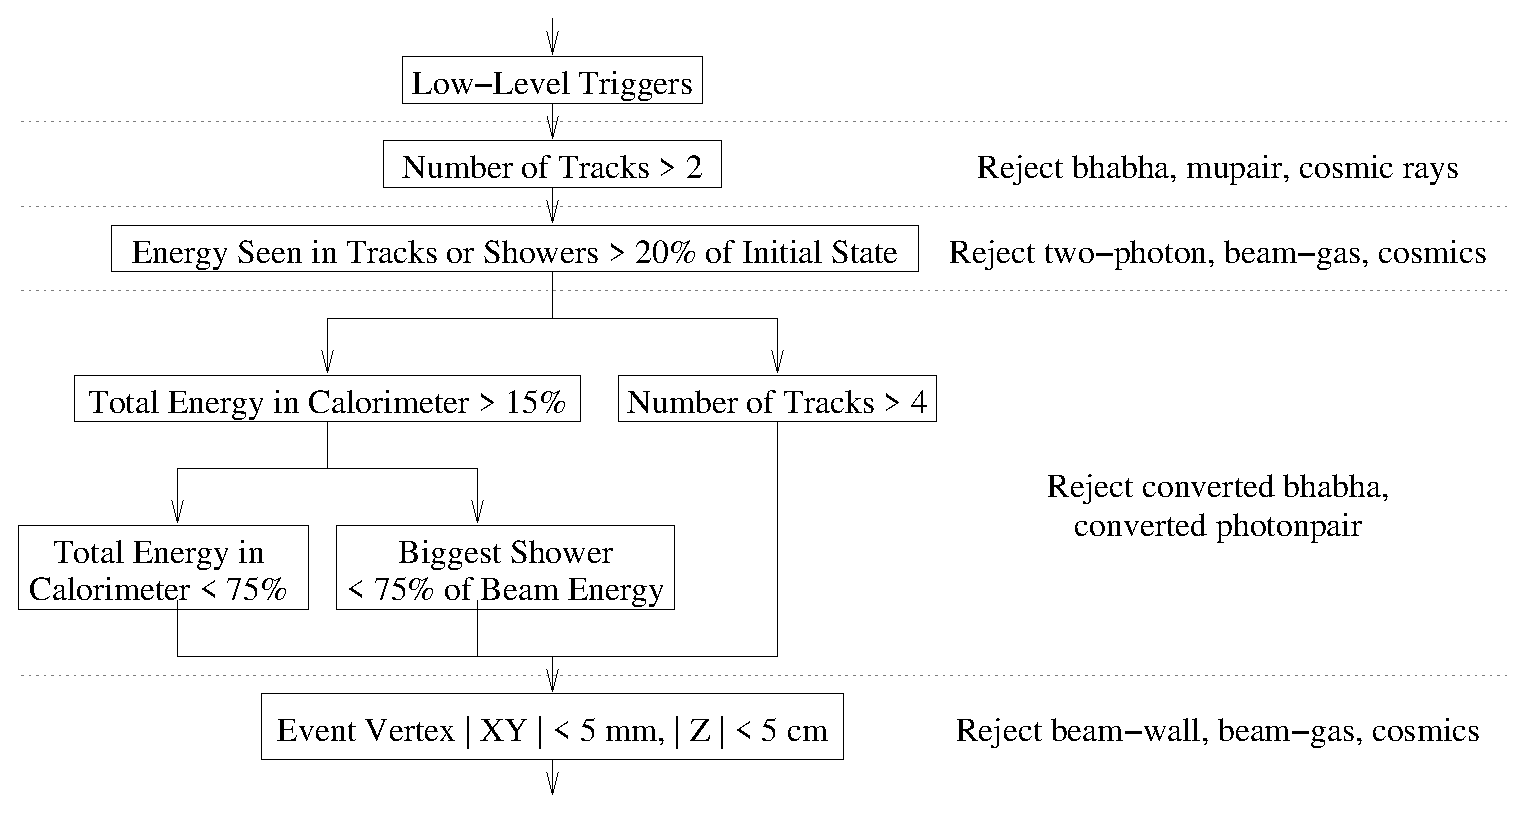
\epsfig{file=cuts.eps, width=\linewidth}
%% \end{center}

\vspace{1 cm}
One selection is not yet well-modelled by Monte Carlo:
\vspace{0.3 cm}
\begin{center}
  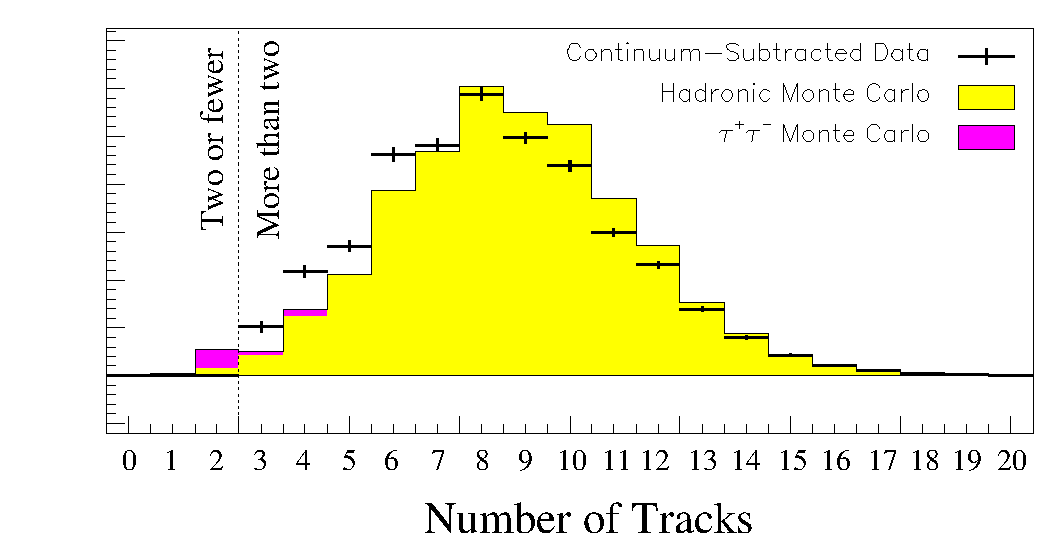
\epsfig{file=datamc_tracks2.eps, width=0.9\linewidth}
%%   \begin{tabular}{p{0.5\linewidth} p{0.43\linewidth}}
%%     \begin{minipage}{\linewidth}
%%       \begin{center}
%%         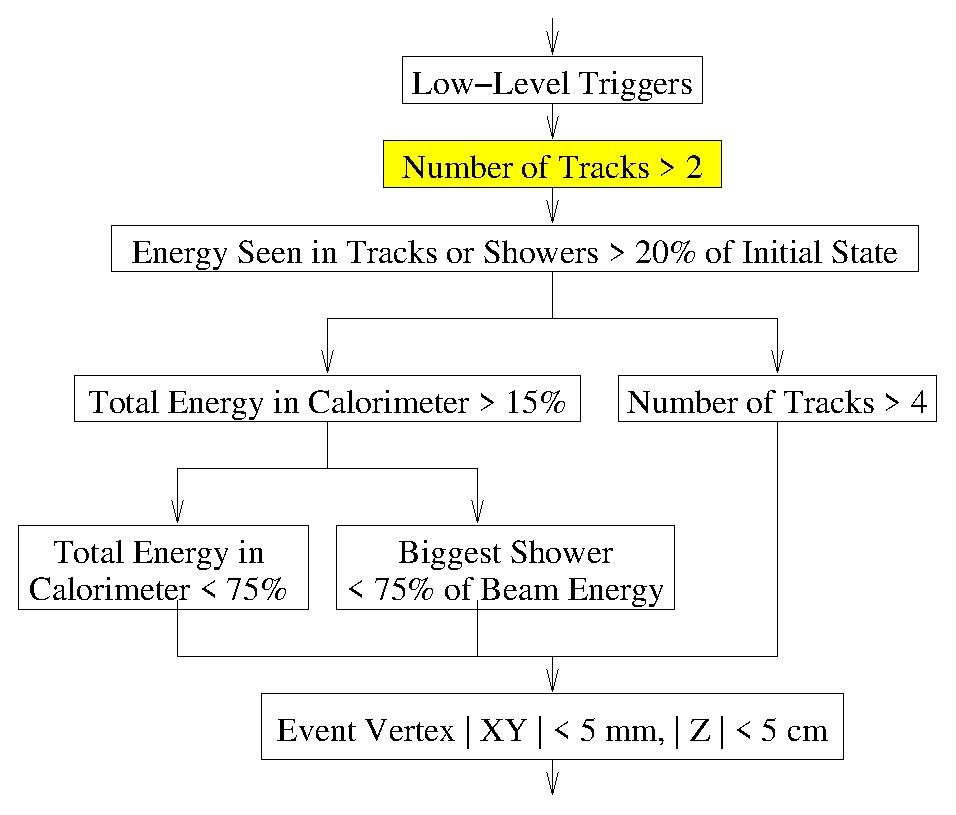
\epsfig{file=cuts2.eps, width=\linewidth}
%%       \end{center}
%%     \end{minipage} &
%%     \begin{minipage}{\linewidth}
%%       \begin{center}
%% 	\vspace{0.3 cm}
%%         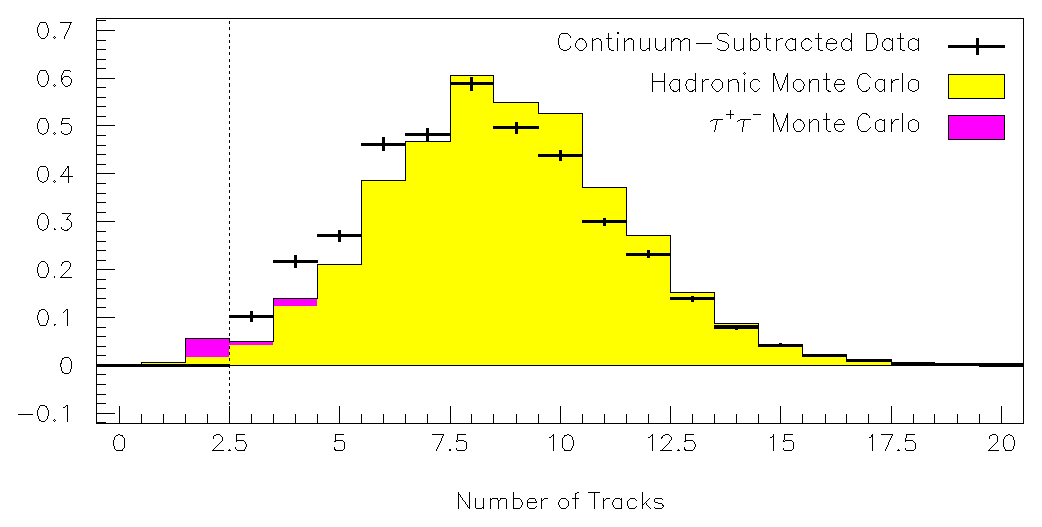
\epsfig{file=datamc_tracks.eps, width=\linewidth}
%%       \end{center}
%%     \end{minipage}
%%   \end{tabular}
\end{center}

\vspace{1 cm}

%% \begin{tabular}{l r r}
%%   M.C.\ Efficiency &
%%   \hspace{0.6 cm} hadrons: 99\% $\pm$ 1\% &
%%   \hspace{0.6 cm} $\tau^+ \tau^-$: 26\% $\pm$ 8\% \\
%% %%   Relevance to \gamee(1S) & $\pm$ 1.0\% & $\pm$ 0.20\% \\
%% %%   Relevance to \gamee(2S) & $\pm$ 1.4\% & $\pm$ 0.10\% \\
%% %%   Relevance to \gamee(3S) & $\pm$ 1.6\% & $\pm$ 0.15\% \\
%% \end{tabular}

\begin{tabular}{l c}
  Monte Carlo efficiency for hadrons: & \hspace{2.45 cm} $\sim$99\% $\pm$ 1\%
\end{tabular}

\vspace{-0.1 cm}
\begin{tabular}{l c c c}
  Relevance to \gamee(1S, 2S, 3S): \hspace{0.7 cm} & $\pm$ 1.0\% & $\pm$ 1.5\% & $\pm$ 1.7\% \\
  Systematic errors $\to$ zero case: & $\pm$ 0.4\% & $\pm$ 0.4\% & $\pm$ 0.5\%
\end{tabular}

%% \vspace{0.8 cm}
%% Plan to reduce systematics by measuring in stages:
%% \vspace{0.2 cm}
%% \begin{center}
%%   \fbox{Monte Carlo} $\longrightarrow$
%%   \fbox{\begin{minipage}{3.5 cm} \centering sample with \\ looser selection \end{minipage}}
%%     $\longrightarrow$
%%   \fbox{this sample}
%% \end{center}

\end{minipage}
\end{slide*}

% %%%%%%%%%%%%%%%%%%%%%%%%%%%%%%%%%%%%%%%%%%%%%%%%%%%%%%%%%%%%%%%%%%%%%%%%%%%

\begin{slide*}
\slideframe{}
\slideframe*[\dkblue]{Oval}
\begin{minipage}[t]{\linewidth}
\Large \black

{
  \dkblue
  \begin{tabular}{c c c c}
    \hspace{0.25 cm} \mbox{Backgrounds} \hspace{0.25 cm} &
    \hspace{0.25 cm} \mbox{Efficiency} \hspace{0.25 cm} &
    \hspace{0.25 cm} \fbox{Luminosity} \hspace{0.25 cm} &
    \hspace{0.25 cm} \mbox{Energy} \hspace{0.25 cm} \\
     & & $\Downarrow$ & \\
  \end{tabular}
}

\vspace{-0.2 cm}
\begin{tabular}{c l}
  $\surd$ & Measured with $e^+e^- \to \gamma \gamma$ \\
  $\rightarrow$ & Measure with $\to e^+e^-$ and $\to \mu^+\mu^-$ also
\end{tabular}

\LARGE

\begin{itemize}

  \item Method: use \cleo\ as a luminosity detector
  \vspace{0.3 cm}
  \begin{flushright}
    \begin{minipage}{0.93\linewidth}
      \begin{enumerate}

        \item Count events with a well-known cross-section
	\begin{minipage}{\linewidth}
	  \hspace{-0.5 cm}
          \begin{tabular}{c c c}
	    \hspace{0.1 cm} $e^+e^- \to e^+e^-$ \hspace{0.1 cm} &
            \hspace{0.1 cm} $e^+e^- \to \mu^+\mu^-$ \hspace{0.1 cm} &
            \hspace{0.1 cm} $e^+e^- \to \gamma\gamma$ \hspace{0.1 cm}
          \end{tabular}
        \end{minipage}

        \item Measure (geometric) acceptance

        \item ${\mathcal L} = N / (\epsilon \, \sigma)$

      \end{enumerate}
    \end{minipage}
  \end{flushright}

  \vspace{0.3 cm}
  \item Only $e^+e^- \to \gamma\gamma$ used so far: 2.5\% systematic error

  \vspace{0.2 cm}
  \item Uncertainty can be reduced by combining all three:
\end{itemize}

\begin{center}
  \fbox{\begin{minipage}{0.9\linewidth}
    \begin{center}
      {\Large \bf Luminosity Measurement with the CLEO II Detector} \\
      Nucl.\ Instrum.\ Meth.\ A {\bf 345}, 429 (1994)
    \end{center}
    \vspace{0.2 cm}
    \begin{abstract}
      A measurement of absolute integrated luminosity is presented
      using the CLEO II detector operating at the CESR $e^+e^-$
      storage ring.  Independent analyses of three different final
      states ($e^+e^-$, $\gamma\gamma$, and $\mu^+\mu^-$) at $\sqrt{s}
      \simeq$10 GeV normalize to the expected theoretical cross
      sections and correct for detection efficiencies.  The resulting
      luminosities are measured with systematic errors of $\pm$1.8\%,
      $\pm$1.6\%, and $\pm$2.2\%, respectively, and are consistent
      with one another. \\
      \epsfig{file=hilight, width=9.1 cm} \vspace{-0.56 cm} \\
      \mbox{The combined luminosity has a systematic error of $\pm$1.0\%.}
    \end{abstract}
  \end{minipage}}
\end{center}

\end{minipage}
\end{slide*}

%%%%%%%%%%%%%%%%%%%%%%%%%%%%%%%%%%%%%%%%%%%%%%%%%%%%%%%%%%%%%%%%%%%%%%%%%%

\begin{slide*}
\slideframe{}
\slideframe*[\dkblue]{Oval}
\begin{minipage}[t]{\linewidth}
\Large \black

{
  \dkblue
  \begin{tabular}{c c c c}
    \hspace{0.25 cm} \mbox{Backgrounds} \hspace{0.25 cm} &
    \hspace{0.25 cm} \mbox{Efficiency} \hspace{0.25 cm} &
    \hspace{0.25 cm} \mbox{Luminosity} \hspace{0.25 cm} &
    \hspace{0.25 cm} \fbox{Energy} \hspace{0.25 cm} \\
     & & & $\Downarrow$ \\
  \end{tabular}
}

\vspace{-0.2 cm}
\begin{tabular}{c l}
  $\surd$ & Scanned each peak many times for cross-checks \\
  $\rightarrow$ & Reduce upper limit on calibration stability \\
\end{tabular}

\LARGE

\vspace{0.25 cm}
\begin{center}
  \begin{tabular}{p{0.02\linewidth} p{0.9\linewidth}}
    \begin{minipage}{\linewidth}
      \rotate[l]{\mbox{$\sigma(e^+e^- \to \mbox{hadrons})$ (nb)}}
    \end{minipage} &
    \begin{minipage}{\linewidth}
      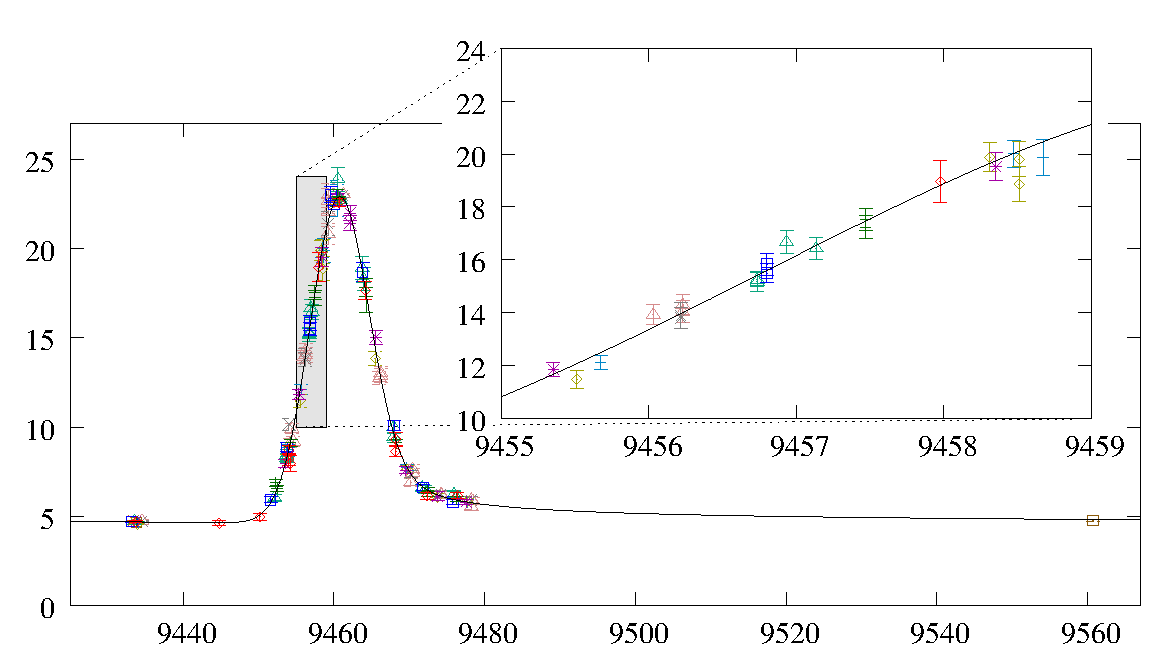
\epsfig{file=high_slope.eps, width=\linewidth}
    \end{minipage} \\
    & \centering Energy (MeV)
  \end{tabular}
\end{center}
\vspace{0.25 cm}

Beam energy measurement is cross-checked by repeating a sample point
at the beginning and end of each scan.

\vspace{0.5 cm}
\begin{tabular}{p{0.75\linewidth} p{0.2\linewidth}}
  \begin{minipage}{\linewidth}
    \begin{flushright}
      Upper limit on energy calibration stability:
    \end{flushright}
  \end{minipage} &
  \begin{minipage}{\linewidth}
    \begin{center}
      \huge 0.2 MeV
    \end{center}
  \end{minipage} \\
  \begin{minipage}{\linewidth}
    \begin{flushright}
      Translated to $\delta(\Gamma_{ee})/\Gamma_{ee}$:
    \end{flushright}
  \end{minipage} &
  \begin{minipage}{\linewidth}
    \begin{center}
      \huge 1.0\%
    \end{center}
  \end{minipage} \\
\end{tabular}

\end{minipage}
\end{slide*}

%%%%%%%%%%%%%%%%%%%%%%%%%%%%%%%%%%%%%%%%%%%%%%%%%%%%%%%%%%%%%%%%%%%%%%%%%%

\begin{slide*}
\slideframe{}
\slideframe*[\dkblue]{Oval}
\heading{\huge Conclusion}
\begin{minipage}[t]{\linewidth}
\LARGE \black

\begin{center}
  \begin{tabular}{l c c c c}
    & \Large \hspace{0.1 cm} $\Gamma_{ee}(1S)$ \hspace{0.1 cm} &
      \Large \hspace{0.1 cm} $\Gamma_{ee}(2S)$ \hspace{0.1 cm} &
      \Large \hspace{0.1 cm} $\Gamma_{ee}(3S)$ \hspace{0.1 cm} &
      \Large $\Gamma_{ee}(2S) / \Gamma_{ee}(1S)$ \\\hline
    \blue Novosibirsk & \blue $\pm$ 3.1\% & \blue $\pm$ 6.4\% & & \blue $\pm$ 4.7\% \\
    \dkgreen this analysis & \dkgreen $\pm$ 2.9\% & \dkgreen $\pm$ 3.1\% & \dkgreen $\pm$ 3.4\% & \dkgreen $\pm$ 2.5\% \\
    \red our goal & \red $\pm$ 1.5\% & \red $\pm$ 1.5\% & \red $\pm$ 1.6\% & \red $\pm$ 1.1\%
  \end{tabular}

  \vspace{0.5 cm}
  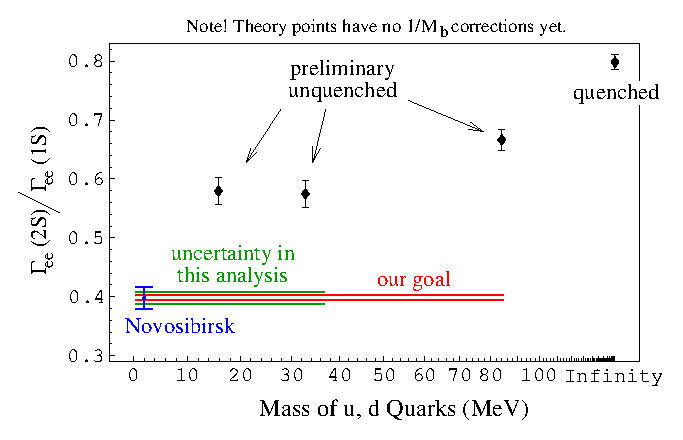
\epsfig{file=conclusion/conclusion.eps, width=\linewidth}
\end{center}

\vspace{0.5 cm} \Large
Theory points by Christine Davies and Alan Gray of the \hpqcd\
collaboration, and used with their permission.  (Thank you!)
\begin{center}
  \fbox{\tt arXiv:hep-lat/0209022}
\end{center}

\end{minipage}
\end{slide*}

%%%%%%%%%%%%%%%%%%%%%%%%%%%%%%%%%%%%%%%%%%%%%%%%%%%%%%%%%%%%%%%%%%%%%%%%%%%

% \begin{slide*}
% \slideframe{}
% \slideframe*[\dkblue]{Oval}
% \begin{minipage}[t]{\linewidth}
% \Large \black

% \end{minipage}
% \end{slide*}

% %%%%%%%%%%%%%%%%%%%%%%%%%%%%%%%%%%%%%%%%%%%%%%%%%%%%%%%%%%%%%%%%%%%%%%%%%%%

% \begin{slide*}
% \slideframe{}
% \slideframe*[\dkblue]{Oval}
% \begin{minipage}[t]{\linewidth}
% \Large \black

% \end{minipage}
% \end{slide*}

% %%%%%%%%%%%%%%%%%%%%%%%%%%%%%%%%%%%%%%%%%%%%%%%%%%%%%%%%%%%%%%%%%%%%%%%%%%%

% \begin{slide*}
% \slideframe{}
% \slideframe*[\dkblue]{Oval}
% \begin{minipage}[t]{\linewidth}
% \Large \black

% \end{minipage}
% \end{slide*}

% %%%%%%%%%%%%%%%%%%%%%%%%%%%%%%%%%%%%%%%%%%%%%%%%%%%%%%%%%%%%%%%%%%%%%%%%%%%

% \begin{slide*}
% \slideframe{}
% \slideframe*[\dkblue]{Oval}
% \begin{minipage}[t]{\linewidth}
% \Large \black

% \end{minipage}
% \end{slide*}

% %%%%%%%%%%%%%%%%%%%%%%%%%%%%%%%%%%%%%%%%%%%%%%%%%%%%%%%%%%%%%%%%%%%%%%%%%%%

% \begin{slide*}
% \slideframe{}
% \slideframe*[\dkblue]{Oval}
% \begin{minipage}[t]{\linewidth}
% \Large \black

% \end{minipage}
% \end{slide*}

% %%%%%%%%%%%%%%%%%%%%%%%%%%%%%%%%%%%%%%%%%%%%%%%%%%%%%%%%%%%%%%%%%%%%%%%%%%%

% \begin{slide*}
% \slideframe{}
% \slideframe*[\dkblue]{Oval}
% \begin{minipage}[t]{\linewidth}
% \Large \black

% \end{minipage}
% \end{slide*}

% %%%%%%%%%%%%%%%%%%%%%%%%%%%%%%%%%%%%%%%%%%%%%%%%%%%%%%%%%%%%%%%%%%%%%%%%%%%

% \begin{slide*}
% \slideframe{}
% \slideframe*[\dkblue]{Oval}
% \begin{minipage}[t]{\linewidth}
% \Large \black

% \end{minipage}
% \end{slide*}

% %%%%%%%%%%%%%%%%%%%%%%%%%%%%%%%%%%%%%%%%%%%%%%%%%%%%%%%%%%%%%%%%%%%%%%%%%%%

% \begin{slide*}
% \slideframe{}
% \slideframe*[\dkblue]{Oval}
% \begin{minipage}[t]{\linewidth}
% \Large \black

% \end{minipage}
% \end{slide*}

% %%%%%%%%%%%%%%%%%%%%%%%%%%%%%%%%%%%%%%%%%%%%%%%%%%%%%%%%%%%%%%%%%%%%%%%%%%%

% \begin{slide*}
% \slideframe{}
% \slideframe*[\dkblue]{Oval}
% \begin{minipage}[t]{\linewidth}
% \Large \black

% \end{minipage}
% \end{slide*}

% %%%%%%%%%%%%%%%%%%%%%%%%%%%%%%%%%%%%%%%%%%%%%%%%%%%%%%%%%%%%%%%%%%%%%%%%%%%

% \begin{slide*}
% \slideframe{}
% \slideframe*[\dkblue]{Oval}
% \begin{minipage}[t]{\linewidth}
% \Large \black

% \end{minipage}
% \end{slide*}

% %%%%%%%%%%%%%%%%%%%%%%%%%%%%%%%%%%%%%%%%%%%%%%%%%%%%%%%%%%%%%%%%%%%%%%%%%%%

% \begin{slide*}
% \slideframe{}
% \slideframe*[\dkblue]{Oval}
% \begin{minipage}[t]{\linewidth}
% \Large \black

% \end{minipage}
% \end{slide*}

% %%%%%%%%%%%%%%%%%%%%%%%%%%%%%%%%%%%%%%%%%%%%%%%%%%%%%%%%%%%%%%%%%%%%%%%%%%%

% \begin{slide*}
% \slideframe{}
% \slideframe*[\dkblue]{Oval}
% \begin{minipage}[t]{\linewidth}
% \Large \black

% \end{minipage}
% \end{slide*}

% %%%%%%%%%%%%%%%%%%%%%%%%%%%%%%%%%%%%%%%%%%%%%%%%%%%%%%%%%%%%%%%%%%%%%%%%%%%

% \begin{slide*}
% \slideframe{}
% \slideframe*[\dkblue]{Oval}
% \begin{minipage}[t]{\linewidth}
% \Large \black

% \end{minipage}
% \end{slide*}

% %%%%%%%%%%%%%%%%%%%%%%%%%%%%%%%%%%%%%%%%%%%%%%%%%%%%%%%%%%%%%%%%%%%%%%%%%%%

% \begin{slide*}
% \slideframe{}
% \slideframe*[\dkblue]{Oval}
% \begin{minipage}[t]{\linewidth}
% \Large \black

% \end{minipage}
% \end{slide*}

% %%%%%%%%%%%%%%%%%%%%%%%%%%%%%%%%%%%%%%%%%%%%%%%%%%%%%%%%%%%%%%%%%%%%%%%%%%%

% \begin{slide*}
% \slideframe{}
% \slideframe*[\dkblue]{Oval}
% \begin{minipage}[t]{\linewidth}
% \Large \black

% \end{minipage}
% \end{slide*}

% %%%%%%%%%%%%%%%%%%%%%%%%%%%%%%%%%%%%%%%%%%%%%%%%%%%%%%%%%%%%%%%%%%%%%%%%%%%

% \begin{slide*}
% \slideframe{}
% \slideframe*[\dkblue]{Oval}
% \begin{minipage}[t]{\linewidth}
% \Large \black

% \end{minipage}
% \end{slide*}

% %%%%%%%%%%%%%%%%%%%%%%%%%%%%%%%%%%%%%%%%%%%%%%%%%%%%%%%%%%%%%%%%%%%%%%%%%%%

% \begin{slide*}
% \slideframe{}
% \slideframe*[\dkblue]{Oval}
% \begin{minipage}[t]{\linewidth}
% \Large \black

% \end{minipage}
% \end{slide*}

% %%%%%%%%%%%%%%%%%%%%%%%%%%%%%%%%%%%%%%%%%%%%%%%%%%%%%%%%%%%%%%%%%%%%%%%%%%%

% \begin{slide*}
% \slideframe{}
% \slideframe*[\dkblue]{Oval}
% \begin{minipage}[t]{\linewidth}
% \Large \black

% \end{minipage}
% \end{slide*}

% %%%%%%%%%%%%%%%%%%%%%%%%%%%%%%%%%%%%%%%%%%%%%%%%%%%%%%%%%%%%%%%%%%%%%%%%%%%

% \begin{slide*}
% \slideframe{}
% \slideframe*[\dkblue]{Oval}
% \begin{minipage}[t]{\linewidth}
% \Large \black

% \end{minipage}
% \end{slide*}

% %%%%%%%%%%%%%%%%%%%%%%%%%%%%%%%%%%%%%%%%%%%%%%%%%%%%%%%%%%%%%%%%%%%%%%%%%%%

% \begin{slide*}
% \slideframe{}
% \slideframe*[\dkblue]{Oval}
% \begin{minipage}[t]{\linewidth}
% \Large \black

% \end{minipage}
% \end{slide*}

% %%%%%%%%%%%%%%%%%%%%%%%%%%%%%%%%%%%%%%%%%%%%%%%%%%%%%%%%%%%%%%%%%%%%%%%%%%%

% \begin{slide*}
% \slideframe{}
% \slideframe*[\dkblue]{Oval}
% \begin{minipage}[t]{\linewidth}
% \Large \black

% \end{minipage}
% \end{slide*}

% %%%%%%%%%%%%%%%%%%%%%%%%%%%%%%%%%%%%%%%%%%%%%%%%%%%%%%%%%%%%%%%%%%%%%%%%%%%

% \begin{slide*}
% \slideframe{}
% \slideframe*[\dkblue]{Oval}
% \begin{minipage}[t]{\linewidth}
% \Large \black

% \end{minipage}
% \end{slide*}

% %%%%%%%%%%%%%%%%%%%%%%%%%%%%%%%%%%%%%%%%%%%%%%%%%%%%%%%%%%%%%%%%%%%%%%%%%%%

% \begin{slide*}
% \slideframe{}
% \slideframe*[\dkblue]{Oval}
% \begin{minipage}[t]{\linewidth}
% \Large \black

% \end{minipage}
% \end{slide*}

% %%%%%%%%%%%%%%%%%%%%%%%%%%%%%%%%%%%%%%%%%%%%%%%%%%%%%%%%%%%%%%%%%%%%%%%%%%%

% \begin{slide*}
% \slideframe{}
% \slideframe*[\dkblue]{Oval}
% \begin{minipage}[t]{\linewidth}
% \Large \black

% \end{minipage}
% \end{slide*}

% %%%%%%%%%%%%%%%%%%%%%%%%%%%%%%%%%%%%%%%%%%%%%%%%%%%%%%%%%%%%%%%%%%%%%%%%%%%

% \begin{slide*}
% \slideframe{}
% \slideframe*[\dkblue]{Oval}
% \begin{minipage}[t]{\linewidth}
% \Large \black

% \end{minipage}
% \end{slide*}

% %%%%%%%%%%%%%%%%%%%%%%%%%%%%%%%%%%%%%%%%%%%%%%%%%%%%%%%%%%%%%%%%%%%%%%%%%%%

% \begin{slide*}
% \slideframe{}
% \slideframe*[\dkblue]{Oval}
% \begin{minipage}[t]{\linewidth}
% \Large \black

% \end{minipage}
% \end{slide*}

% %%%%%%%%%%%%%%%%%%%%%%%%%%%%%%%%%%%%%%%%%%%%%%%%%%%%%%%%%%%%%%%%%%%%%%%%%%%

% \begin{slide*}
% \slideframe{}
% \slideframe*[\dkblue]{Oval}
% \begin{minipage}[t]{\linewidth}
% \Large \black

% \end{minipage}
% \end{slide*}

% %%%%%%%%%%%%%%%%%%%%%%%%%%%%%%%%%%%%%%%%%%%%%%%%%%%%%%%%%%%%%%%%%%%%%%%%%%%

% \begin{slide*}
% \slideframe{}
% \slideframe*[\dkblue]{Oval}
% \begin{minipage}[t]{\linewidth}
% \Large \black

% \end{minipage}
% \end{slide*}

% %%%%%%%%%%%%%%%%%%%%%%%%%%%%%%%%%%%%%%%%%%%%%%%%%%%%%%%%%%%%%%%%%%%%%%%%%%%

% \begin{slide*}
% \slideframe{}
% \slideframe*[\dkblue]{Oval}
% \begin{minipage}[t]{\linewidth}
% \Large \black

% \end{minipage}
% \end{slide*}

% %%%%%%%%%%%%%%%%%%%%%%%%%%%%%%%%%%%%%%%%%%%%%%%%%%%%%%%%%%%%%%%%%%%%%%%%%%%

% \begin{slide*}
% \slideframe{}
% \slideframe*[\dkblue]{Oval}
% \begin{minipage}[t]{\linewidth}
% \Large \black

% \end{minipage}
% \end{slide*}

% %%%%%%%%%%%%%%%%%%%%%%%%%%%%%%%%%%%%%%%%%%%%%%%%%%%%%%%%%%%%%%%%%%%%%%%%%%%

% \begin{slide*}
% \slideframe{}
% \slideframe*[\dkblue]{Oval}
% \begin{minipage}[t]{\linewidth}
% \Large \black

% \end{minipage}
% \end{slide*}

% %%%%%%%%%%%%%%%%%%%%%%%%%%%%%%%%%%%%%%%%%%%%%%%%%%%%%%%%%%%%%%%%%%%%%%%%%%%

% \begin{slide*}
% \slideframe{}
% \slideframe*[\dkblue]{Oval}
% \begin{minipage}[t]{\linewidth}
% \Large \black

% \end{minipage}
% \end{slide*}

% %%%%%%%%%%%%%%%%%%%%%%%%%%%%%%%%%%%%%%%%%%%%%%%%%%%%%%%%%%%%%%%%%%%%%%%%%%%

% \begin{slide*}
% \slideframe{}
% \slideframe*[\dkblue]{Oval}
% \begin{minipage}[t]{\linewidth}
% \Large \black

% \end{minipage}
% \end{slide*}

% %%%%%%%%%%%%%%%%%%%%%%%%%%%%%%%%%%%%%%%%%%%%%%%%%%%%%%%%%%%%%%%%%%%%%%%%%%%

% \begin{slide*}
% \slideframe{}
% \slideframe*[\dkblue]{Oval}
% \begin{minipage}[t]{\linewidth}
% \Large \black

% \end{minipage}
% \end{slide*}

% %%%%%%%%%%%%%%%%%%%%%%%%%%%%%%%%%%%%%%%%%%%%%%%%%%%%%%%%%%%%%%%%%%%%%%%%%%%

% \begin{slide*}
% \slideframe{}
% \slideframe*[\dkblue]{Oval}
% \begin{minipage}[t]{\linewidth}
% \Large \black

% \end{minipage}
% \end{slide*}

% %%%%%%%%%%%%%%%%%%%%%%%%%%%%%%%%%%%%%%%%%%%%%%%%%%%%%%%%%%%%%%%%%%%%%%%%%%%

% \begin{slide*}
% \slideframe{}
% \slideframe*[\dkblue]{Oval}
% \begin{minipage}[t]{\linewidth}
% \Large \black

% \end{minipage}
% \end{slide*}

% %%%%%%%%%%%%%%%%%%%%%%%%%%%%%%%%%%%%%%%%%%%%%%%%%%%%%%%%%%%%%%%%%%%%%%%%%%%

% \begin{slide*}
% \slideframe{}
% \slideframe*[\dkblue]{Oval}
% \begin{minipage}[t]{\linewidth}
% \Large \black

% \end{minipage}
% \end{slide*}

% %%%%%%%%%%%%%%%%%%%%%%%%%%%%%%%%%%%%%%%%%%%%%%%%%%%%%%%%%%%%%%%%%%%%%%%%%%%

% \begin{slide*}
% \slideframe{}
% \slideframe*[\dkblue]{Oval}
% \begin{minipage}[t]{\linewidth}
% \Large \black

% \end{minipage}
% \end{slide*}

% %%%%%%%%%%%%%%%%%%%%%%%%%%%%%%%%%%%%%%%%%%%%%%%%%%%%%%%%%%%%%%%%%%%%%%%%%%%

% \begin{slide*}
% \slideframe{}
% \slideframe*[\dkblue]{Oval}
% \begin{minipage}[t]{\linewidth}
% \Large \black

% \end{minipage}
% \end{slide*}

% %%%%%%%%%%%%%%%%%%%%%%%%%%%%%%%%%%%%%%%%%%%%%%%%%%%%%%%%%%%%%%%%%%%%%%%%%%%

% \begin{slide*}
% \slideframe{}
% \slideframe*[\dkblue]{Oval}
% \begin{minipage}[t]{\linewidth}
% \Large \black

% \end{minipage}
% \end{slide*}

% %%%%%%%%%%%%%%%%%%%%%%%%%%%%%%%%%%%%%%%%%%%%%%%%%%%%%%%%%%%%%%%%%%%%%%%%%%%

% \begin{slide*}
% \slideframe{}
% \slideframe*[\dkblue]{Oval}
% \begin{minipage}[t]{\linewidth}
% \Large \black

% \end{minipage}
% \end{slide*}

% %%%%%%%%%%%%%%%%%%%%%%%%%%%%%%%%%%%%%%%%%%%%%%%%%%%%%%%%%%%%%%%%%%%%%%%%%%%

% \begin{slide*}
% \slideframe{}
% \slideframe*[\dkblue]{Oval}
% \begin{minipage}[t]{\linewidth}
% \Large \black

% \end{minipage}
% \end{slide*}

% %%%%%%%%%%%%%%%%%%%%%%%%%%%%%%%%%%%%%%%%%%%%%%%%%%%%%%%%%%%%%%%%%%%%%%%%%%%

\end{document}

